%%%%%%%%%%%%%%%%%%%%%%%%%%%%%%%%%%%%%%%%%%%%%%%%%%%%%%%%%%%%%%%%%%%%%%%%%%%%%%%%
%2345678901234567890123456789012345678901234567890123456789012345678901234567890
%        1         2         3         4         5         6         7         8

\documentclass[letterpaper, 10 pt, conference]{ieeeconf}  % Comment this line out if you need a4paper

%\documentclass[a4paper, 10pt, conference]{ieeeconf}      % Use this line for a4 paper

%\IEEEoverridecommandlockouts                              % This command is only needed if 
                                                          % you want to use the \thanks command

\overrideIEEEmargins                                      % Needed to meet printer requirements.

% See the \addtolength command later in the file to balance the column lengths
% on the last page of the document

% The following packages can be found on http:\\www.ctan.org
\usepackage{graphics} % for pdf, bitmapped graphics files
\usepackage{epsfig} % for postscript graphics files
\usepackage{mathptmx} % assumes new font selection scheme installed
\usepackage{times} % assumes new font selection scheme installed
\usepackage{amsmath} % assumes amsmath package installed
\usepackage{amssymb}  % assumes amsmath package installed

% Added suport for bibtext files.
\usepackage[backend=biber]{biblatex}
\addbibresource{biblatex-ela427.bib}

% --- packages for drawing diagrams----
\usepackage{tikz}
\usetikzlibrary{arrows,automata}
% --- end state -------------------------

% OBS Newer ever..

% Package that forces figures to stai within the section.
\usepackage[section]{placeins}

%package for utf-8 support
\usepackage[utf8]{inputenc}

%colour
\usepackage{color}
\graphicspath{ {images/}{mesurment/data} }

%Captions
\usepackage[justification=centering,font=small,labelfont=bf]{caption}
\usepackage{hyperref}
\usepackage{url}


\title{\LARGE \bf
LIDAR project report in ELA427}
\author{Hampus Baaz, Magnus \"{O}stgren and Magnus S\"{o}rensen }
\begin{document}

\maketitle
\thispagestyle{empty}
\pagestyle{empty}

%%%%%%%%%%%%%%%%%%%%%%%%%%%%%%%%%%%%%%%%%%%%%%%%%%%%%%%%%%%%%%%%%%%%%%%%%%%%%%%%
\begin{abstract}
This is an report for the course ELA427 at M\"{a}rlardalen university. The aim of the project is to create a LIDAR and report on its behaviors.\\
\textcolor{red}{Nu ska jag inte komma och bråka, men detta låter mer som introduction än abstract, och abstract skrivs oftast och enklast sist.} Men, bara tips, inte klagomål, och jag ska såklart också hjälpa till.. ska bara bli klar med alla mina tentor 
\end{abstract}


%%%%%%%%%%%%%%%%%%%%%%%%%%%%%%%%%%%%%%%%%%%%%%%%%%%%%%%%%%%%%%%%%%%%%%%%%%%%%%%%
\section{INTRODUCTION}
%Example for siting remove when not needed. ~\cite{wikibook}.




%%%%%%%%%%%%%%%%%%%%%%%%%%%%%%%%%%%%%%%%%%%%%%%%%%%%%%%%%%%%%%%%%%%%%%%%%%%%%%%%
\section{HARDWARE}
%Here is all the information about the hardware
The hardware is built to exceed the requirement for the current motor and also be able to control more powerful equipment. \newline
The hardware is built up by 2 H-bridges, sharp 2Y0A21F IR snesor, NI myRIO, 42BYGHM809 Bipolar stepper motor and a LM2596 DC-DC buck converter. 
Each H-bridge have a pair of high power, high voltage N and P MOSFETs (2 of each) which need 10V to open. 4 optocouplers provide the MOSFETs with a high voltage line (of 10+V) to open since the voltage to the stepper motor is only 3.3V. The optocouplers also provide galvanic isolation between the expensive myRIO and the high power motor control. On the digital side (where the myRIO is connected) there is a 75
%If however a 10+V motor is used the DC-DC buck would not be needed since its function is to only to provide the possibility to have one pair of cables from the power supply. 
High power motors also create a lot of noise and therefor there is two pairs of capacitors. One 100µF and one smaller 1µF to smooth out different types of noise. There is one pair of capacitor on each powerline (motor power and mosfet power)

\section{Software}
% Magnus S fixar detta
%In this LIDAR lab oration the National instruments myRIO was used in combination with National instruments LabWIEV. 
When using myRIO as an base for the LIDAR there is a coupel of design considerations to take in to count especially if the LIDAR have the need to be fast because then the latency and the transfer speed of the USB can be a limitation. 
In this project it was decided to go with an spitted architecture letting the myRIO do the measurements and controlling the motor while the personal computer was used to display the data that the myRIO captured.

\subsection{The myRIO software}\label{subsection:myRIO}
\begin{figure}[ht]
    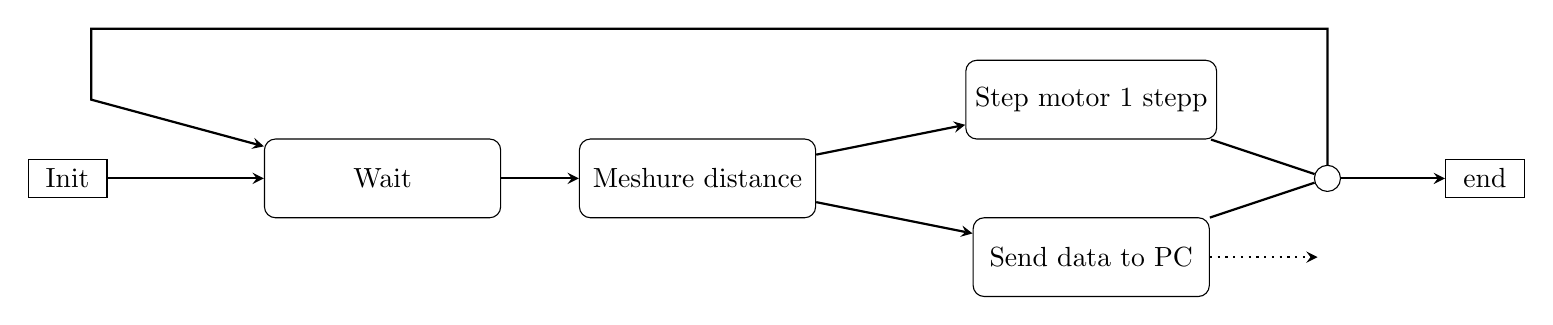
\begin{tikzpicture}
\tikzstyle{startstop} = [rectangle, rounded corners , minimum width=3cm, minimum height=1cm,text centered, draw=black]
\tikzstyle{round}=[circle, minimum width=0cm,draw=black]
\tikzstyle{first} = [rectangle, minimum width=1cm, draw=black]
\tikzstyle{empty}=[]

\usetikzlibrary{shapes.geometric, arrows}
\tikzstyle{arrow} = [thick,->,>=stealth]
\tikzstyle{dottarrow} = [thick, dotted,->,>=stealth]
\tikzstyle{noarrow}=[thick,-=,=stealth]

%nodes
\node (init) [first] {Init};
\node (wait) [startstop, right of =init, xshift=3cm] {Wait};
\node (mesh) [startstop, right of=wait, xshift=3cm] {Meshure distance};
\node (step) [startstop, right of=mesh, xshift=4cm ,yshift=1cm] {Step motor 1 stepp};
\node (send) [startstop, below of=step, yshift=-1cm]{Send data to PC};
\node (merge) [round, right of=send, yshift=1cm, xshift=2cm]{};
\node (end) [first, right of=merge, xshift=1cm] {end};
\node (topc) [empty, right of=send, xshift=2cm]{};

%arrows
\draw [arrow] (wait) -- (mesh);
\draw [arrow] (init) -- (wait);
\draw [arrow] (mesh) -- (step);
\draw [arrow] (mesh) -- (send);
\draw [noarrow] (send) -- (merge);
\draw [noarrow] (step) -- (merge);
\draw [dottarrow] (send) -- (topc);
\draw [arrow] (merge)  -- +(0,1.9)  -- (0.3,1.9) -- (0.3,1) -- (wait);
\draw [arrow] (merge) -- (end);
\end{tikzpicture}
  \caption{This figure describes the inner simplified working of the myRIO code.
  At initialise we initialise the unit. Then because how the myRIO is working the code is waiting while the myRIO is measuring the sensor. The measure block only represents that we retrieve the value of the previously measured data. The data is put on the FIFO stack to b sent to the computer while myRIO takes an other step with the stepper motor. When that is done and the user haven't pressed stop to abort we loop back to wait and do the measurement again.}
  \label{fig:myRIO-loop}
\end{figure}
The myRIO part of the code uses an loop described in figure \ref{fig:myRIO-loop}.

\subsubsection{Measuring data}\label{subsubsection:mesure}
The implementation of myRIO reads the data continuously.
And therefore the motor needs to stop before the read block reads the value.
After the value have bin acquired the system stores the value as $y$ with the motor position $x$ in to an an cluster and then in to an array of clusters. In this case the the motor mentioned in \ref{section:hardware} have 400 steps and therefor the size of that array is 400 elements.

\subsubsection{Sending data to pc}\label{subsubsection:sendData}
The array previously mentioned in the section \ref{subsubsection:mesure} is sent over an network based shared variable that is implemented as an first in first out queue\cite{myRIO-Shared}. 


\subsubsection{Step motor control}\label{subsubsection:Step-control}
Step motor control is achieved by using a implementation of a shift register explained in figure \ref{fig:shift-reg}. 

\begin{figure}[ht]
  \centering
  \begin{tikzpicture}
\tikzstyle{notused} = [rectangle, rounded corners , minimum width=3mm, minimum height=1mm,text centered, draw=black]
\tikzstyle{round}=[circle, minimum width=0mm,draw=black]
\tikzstyle{square} = [rectangle, minimum width=1mm, draw=black]
\tikzstyle{empty}=[]

\usetikzlibrary{shapes.geometric, arrows}
\tikzstyle{arrow} = [thick,->,>=stealth]
\tikzstyle{dottarrow} = [thick, dotted,->,>=stealth]
\tikzstyle{noarrow}=[thick,-=,=stealth]

%node
\node (DA) [square] {T};
\node (DB) [square, right of =DA, xshift=-6mm] {F};
\node (DC) [square, right of =DB, xshift=-6mm] {F};
\node (DD) [square, right of =DC, xshift=-6mm] {F};

\node (DE) [square, right of =DD, xshift=0mm] {F};
\node (DF) [square, right of =DE, xshift=-6mm] {T};
\node (DG) [square, right of =DF, xshift=-6mm] {F};
\node (DH) [square, right of =DG, xshift=-6mm] {F};

%Epmty target nodes
\node (DAT) [empty, top of=DA, yshift=8mm]{}
\node (DBT) [empty, top of=DB, yshift=8mm]{}
\node (DCT) [empty, top of=DC, yshift=8mm]{}
\node (DDT) [empty, top of=DD, yshift=8mm]{}

\node (DET) [empty, top of=DE, yshift=8mm]{}
\node (DFT) [empty, top of=DF, yshift=8mm]{}
\node (DGT) [empty, top of=DG, yshift=8mm]{}
\node (DHT) [empty, top of=DH, yshift=8mm]{}

%lines to target node
\draw [arrow] (DA) -- (DAT);
%node (D1) [square right of=Dfirst, xshift=8mm] {F};
%\node (D2) [square right of=D1, xshift=8mm] {F};
\end{tikzpicture}
  \caption{The shift register is working by step wise shifting the true state on step to the right and in this case have output upward. In this case the register is in state 1 at the left and proceed in the direction of the dotted arrow when moving over to the next state. When the true state reaches the right most cell it will on the next step be shifted to the beginning of the register. The output of this register is a 4 bit pararell bus denoted by the up facing arrows.}
  \label{fig:shift-reg}
\end{figure}
The motor is then pair wise connected to the each bit in the shift register thus implementing wave drive.

\subsection{Computer side}\label{subsection:computer-side}
The computer receives the data from the myRIO device and renders the result on the screen. In the figure \ref{fig:data-recive} a demonstration of the proces can be shown.

\begin{figure}[ht]
    \centering
   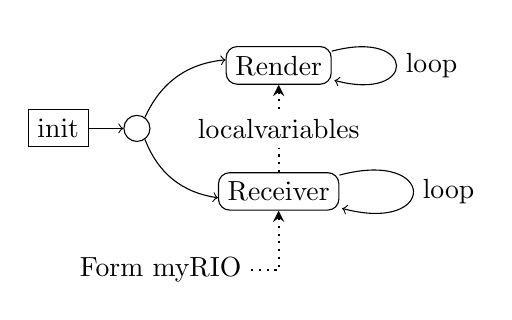
\begin{tikzpicture}
\tikzstyle{rounded} = [rectangle, rounded corners , minimum width=3mm, minimum height=1mm,text centered, draw=black]
\tikzstyle{round}=[circle, minimum width=0mm,draw=black]
\tikzstyle{square} = [rectangle, minimum width=1mm, draw=black]
\tikzstyle{empty}=[]

\usetikzlibrary{shapes.geometric, arrows}
\tikzstyle{arrow} = [thick,->,>=stealth]
\tikzstyle{dottarrow} = [thick, dotted,->,>=stealth]
\tikzstyle{dottline} = [thick, dotted,-,>=stealth]
\tikzstyle{noarrow}=[thick,-=,=stealth]

%nodes
\node (init) [square] {init};
\node (loop) [round, right of=init]{};
\node (render)[rounded, right of=loop, xshift=8mm, yshift=8mm ] {Render};
\node (rezive) [rounded, right of=loop, xshift=8mm, yshift=-8mm] {Receiver};
\node (datain) [empty, below of=rezive, xshift=-15mm]{Form myRIO};
\node (shared) [empty, below of=render, yshift=2mm]{localvariables};


%lines
%(Startnode)  edge [bend arrow]       node[text pos]  {text}          (target);
\path[->] 
(init) 		edge 								node[left]		{}			(loop)
(loop)		edge[bend left] 					node[left]		{}			(render)
(loop)		edge[bend right]					node[left]		{}			(rezive)
(render) 	edge[loop right]					node[right]		{loop}			(render)
(rezive) 	edge[loop right]					node[right]		{loop}			(rezive)
;
\draw [dottarrow] (datain) -| (rezive);
%\draw [dottarrow] (rezive) -- (render);
\draw [dottline] (rezive) -- (shared);
\draw [dottarrow] (shared) -- (render);

\end{tikzpicture}
  \caption{When the computer is runs the code. It first goes throw an initialisation phase that sets some common variables. After that it splits in 2 threads for with one is responsible for collecting the data from the myRIO and the other thread have the responsibility of rendering the user interface and the different graphical element.}
  \label{fig:data-recive}
\end{figure}

\subsubsection{Collecting the data form myRIO}\label{subsubsection:collectData}
Sins the myRIO sends the data in an array of clusters the program needs to extract the data in each $y$ value and convert the value that is based on voltage to an value that is based on distance. That conversion is done doing an exponential regression over value and range, more info about the regression can be found in chapter \ref{secition:results}. The compute then stores the cluster array in memory so it can be sent over to the other loop by using local variables. 

\subsubsection{Rendering the Polar-plot}\label{subsubsection:renderPolar}
Rendering the polar plot is then done by sending that array in to the polar plot with point iteration\cite{labVIEW-polar-plot} in the render thread. 
This is done because then render can run in a slower phase then the receiver and thus save decrees the power usage of the program. 
As an side effect of this the screen is much more stable and don't blink as much.

\subsubsection{Computing the histogram}\label{subsubsection:comphistogram}
This program have a ability to generate a histogram view of the length based users inputed expected value defined as $\mu:=$"User expected value" and delta value $\Delta:=$"Users expected min/max" that is going to be used to calculated an expected min and max value defined as $ max:=\mu+\Delta,\quad min:=\mu-\Delta, \quad D:=$"Distance to object".
The computation is done by first taking each measurement and checking if the value of the data is in the interval of $ (min \leq D \leq max) $ then if so restore the data as an frequency array by using the distance as indexer in the array and increasing the value in that cell by one.
Value that ocurs outside the expeted min/max interval is ignored.
In this way the histogram plot even works for detecting mean and standard deviation while rotating in \textbf{non} deterministic environment.
Then from the frequency array we created ealier the program can calculate mean and standard deviation by using the formulas.
$$\begin{matrix} 
\overline{x}=\frac{\Sigma(x_i-\mu)^2}{\Sigma(y_i)} & 
\sigma= \sqrt{\frac{\Sigma((f_i*x_i-\overline{x})^2)}{\Sigma(f_i)}}
\end{matrix}\label{equation:mean-and-div}$$
Finaly the figure is rendered using labVIEWs "plot waveform vi" \cite{labVIEW-Plot-Waveform-VI} by also taking the max value and min value as an argument in to the plot. 

\section{Measurement and test results}
% Magnus S fixar detta
%
\section{Test set up}\label{section:testSetUp}
The measurement for this LIDAr was done by measuring the distance between  the sensor and an target, both rotating and while standstill (static) for to acquire the necessary data. Figure \ref{fig:testSetUp} describes how the test set up was done.
%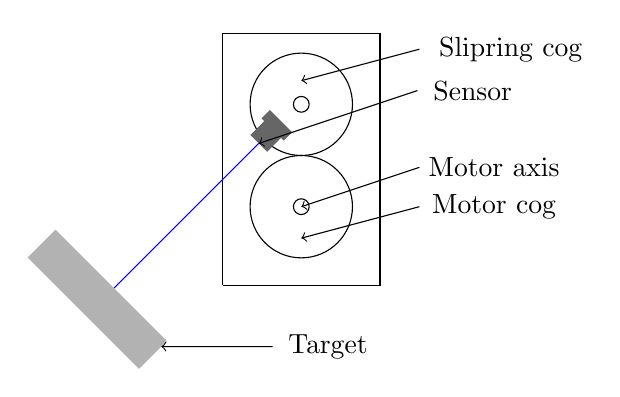
\begin{tikzpicture}[xscale=0.5, yscale=0.5]
\draw (0,0) -- (4,0) -- (4,6.4) -- (0,6.4) -- (0,0); %outre box
\draw (2,2) circle (1.3); %cog for motor
\draw (2,2) circle (0.2); % axis for motor
\draw (2,4.6) circle (1.3); %cog for slipring
\draw (2,4.6) circle (0.2); %axis for silp ring

%Sensor of the top cog
\fill[black!60!white, rotate=-45] (-2.3,4.0) rectangle (-1.5,3.7);
\fill[black!60!white, rotate=-45] (-2.2,3.2) rectangle (-1.6,3.8);
%beeam
\draw[blue, rotate=-45] (-1.9,3.2) -- (-1.9,-2);
%target
\fill[black!30!white, rotate=-45] (-4,-2) rectangle (0,-3);

%arrows
\draw[->, rotate=-45] (0,7)node[xshift=20] {Sensor} -- (-1.9,3.2);
\draw[->] (5,3)node[xshift=27] {Motor axis} -- (2.0,2.0) ;% motor axis
\draw[->] (5,2)node[xshift=27] {Motor cog} -- (2.0,1.2);% motor cog
\draw[->] (5,6)node[xshift=33] {Slipring cog} -- (2.0,5.2);% lidar cog
\draw[->, rotate=-45] (2,-0.2)node[xshift=20] {Target} -- (-0.0,-2.2);

\end{tikzpicture}
\begin{figure}[ht]
    \centering
   %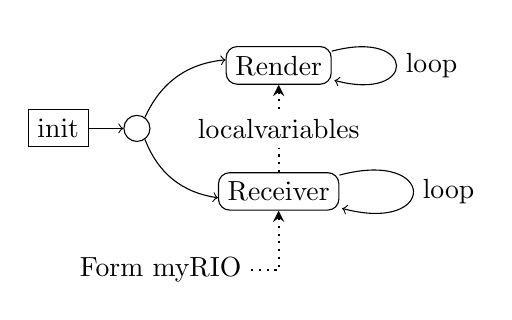
\begin{tikzpicture}
\tikzstyle{rounded} = [rectangle, rounded corners , minimum width=3mm, minimum height=1mm,text centered, draw=black]
\tikzstyle{round}=[circle, minimum width=0mm,draw=black]
\tikzstyle{square} = [rectangle, minimum width=1mm, draw=black]
\tikzstyle{empty}=[]

\usetikzlibrary{shapes.geometric, arrows}
\tikzstyle{arrow} = [thick,->,>=stealth]
\tikzstyle{dottarrow} = [thick, dotted,->,>=stealth]
\tikzstyle{dottline} = [thick, dotted,-,>=stealth]
\tikzstyle{noarrow}=[thick,-=,=stealth]

%nodes
\node (init) [square] {init};
\node (loop) [round, right of=init]{};
\node (render)[rounded, right of=loop, xshift=8mm, yshift=8mm ] {Render};
\node (rezive) [rounded, right of=loop, xshift=8mm, yshift=-8mm] {Receiver};
\node (datain) [empty, below of=rezive, xshift=-15mm]{Form myRIO};
\node (shared) [empty, below of=render, yshift=2mm]{localvariables};


%lines
%(Startnode)  edge [bend arrow]       node[text pos]  {text}          (target);
\path[->] 
(init) 		edge 								node[left]		{}			(loop)
(loop)		edge[bend left] 					node[left]		{}			(render)
(loop)		edge[bend right]					node[left]		{}			(rezive)
(render) 	edge[loop right]					node[right]		{loop}			(render)
(rezive) 	edge[loop right]					node[right]		{loop}			(rezive)
;
\draw [dottarrow] (datain) -| (rezive);
%\draw [dottarrow] (rezive) -- (render);
\draw [dottline] (rezive) -- (shared);
\draw [dottarrow] (shared) -- (render);

\end{tikzpicture}
   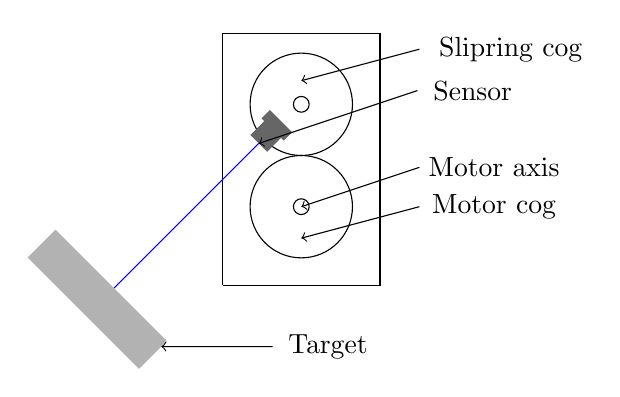
\begin{tikzpicture}[xscale=0.5, yscale=0.5]
\draw (0,0) -- (4,0) -- (4,6.4) -- (0,6.4) -- (0,0); %outre box
\draw (2,2) circle (1.3); %cog for motor
\draw (2,2) circle (0.2); % axis for motor
\draw (2,4.6) circle (1.3); %cog for slipring
\draw (2,4.6) circle (0.2); %axis for silp ring

%Sensor of the top cog
\fill[black!60!white, rotate=-45] (-2.3,4.0) rectangle (-1.5,3.7);
\fill[black!60!white, rotate=-45] (-2.2,3.2) rectangle (-1.6,3.8);
%beeam
\draw[blue, rotate=-45] (-1.9,3.2) -- (-1.9,-2);
%target
\fill[black!30!white, rotate=-45] (-4,-2) rectangle (0,-3);

%arrows
\draw[->, rotate=-45] (0,7)node[xshift=20] {Sensor} -- (-1.9,3.2);
\draw[->] (5,3)node[xshift=27] {Motor axis} -- (2.0,2.0) ;% motor axis
\draw[->] (5,2)node[xshift=27] {Motor cog} -- (2.0,1.2);% motor cog
\draw[->] (5,6)node[xshift=33] {Slipring cog} -- (2.0,5.2);% lidar cog
\draw[->, rotate=-45] (2,-0.2)node[xshift=20] {Target} -- (-0.0,-2.2);

\end{tikzpicture}
  \caption{The LIDAR had the construction with an slip ring to allow free passage of the cable without being twinned. Therefore it used 2 3D printed cogs to transfer the rotation from the motor to the sensor. The lower circle describe the cog that was connected to the motor whiles the top one with the sensor describe the cog that had an slip ring in it. There are also an target to the bottom left, how ever the distance is not up to scale hear for spacing reason.}
  \label{fig:testSetUp}
\end{figure}

\section{Measurement and test results}\label{secition:results}
The measurements that was taken for this report was done both while the motor was rotating and standing still (static). And are represented as polar plots and histogram of the distance. 

\subsection{Smallest detectable object}\label{subsection:mesurment-smalest}
The smallest object that the sensor can detect is dependent on zise of the object, speed of the LIDAR and distance between the LIDAR and the object.

In our test we tested with an round object that had a diameter of $6mm$. 
After a series of test the conclusion was that it could see the object in between $113mm$ and $300mm$ when the delay was $40ms$ in between each step.
If the step delay adjusted down to $1ms$ the LIDAR was still able to detect it sometimes and the range decreased to below $230mm$.


\subsection{Minimum speed}\label{subsetion:mesurmen-miniSpeed}
The minimum speed was also dependent on in with direction the object travelled in relation to the LIDAR. 
Al test was done with an one meter long wooden plank that was hanging from a string so it could be easy manipulated.
When the object approached the LIDAR that was rotating with an delay of $1.5ms$ against the LIDARs beam the measurement showed that the object wasent detecteble if the object moved faster then $1m/s$. 
The other direction gave the result $0.4m/s$ dependent a bit of the initial position.

\subsection{Different objects}\label{subsection:mesurment-difObj}
The test that was preformed was if the LIDAR could see an transparent acrylic box.
And the data suggested it wasn't any big difference between the box and the solid object. 
Highly reflective material was only captured when it was almost orgogonal to the object.

\subsection{The sensors accuracy}\label{subsubsection:accuracy}
Data for the sensors accuracy was obtained by using the function described earlier in section \ref{subsubsection:comphistogram}. The data that was captured is as shown in figure \ref{fig:test-hist}.

\begin{figure}[ht]
    \centering
   %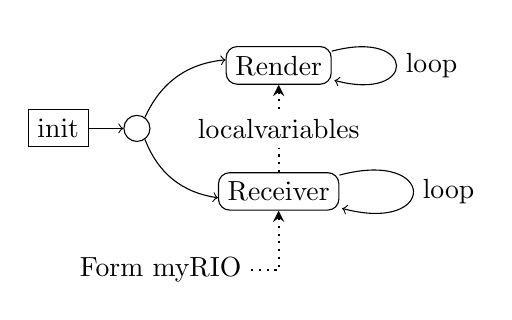
\begin{tikzpicture}
\tikzstyle{rounded} = [rectangle, rounded corners , minimum width=3mm, minimum height=1mm,text centered, draw=black]
\tikzstyle{round}=[circle, minimum width=0mm,draw=black]
\tikzstyle{square} = [rectangle, minimum width=1mm, draw=black]
\tikzstyle{empty}=[]

\usetikzlibrary{shapes.geometric, arrows}
\tikzstyle{arrow} = [thick,->,>=stealth]
\tikzstyle{dottarrow} = [thick, dotted,->,>=stealth]
\tikzstyle{dottline} = [thick, dotted,-,>=stealth]
\tikzstyle{noarrow}=[thick,-=,=stealth]

%nodes
\node (init) [square] {init};
\node (loop) [round, right of=init]{};
\node (render)[rounded, right of=loop, xshift=8mm, yshift=8mm ] {Render};
\node (rezive) [rounded, right of=loop, xshift=8mm, yshift=-8mm] {Receiver};
\node (datain) [empty, below of=rezive, xshift=-15mm]{Form myRIO};
\node (shared) [empty, below of=render, yshift=2mm]{localvariables};


%lines
%(Startnode)  edge [bend arrow]       node[text pos]  {text}          (target);
\path[->] 
(init) 		edge 								node[left]		{}			(loop)
(loop)		edge[bend left] 					node[left]		{}			(render)
(loop)		edge[bend right]					node[left]		{}			(rezive)
(render) 	edge[loop right]					node[right]		{loop}			(render)
(rezive) 	edge[loop right]					node[right]		{loop}			(rezive)
;
\draw [dottarrow] (datain) -| (rezive);
%\draw [dottarrow] (rezive) -- (render);
\draw [dottline] (rezive) -- (shared);
\draw [dottarrow] (shared) -- (render);

\end{tikzpicture}
        \includegraphics[scale=0.2] {./mesurment/data/Expected_170,0__Mean_176,02__Distrubution_13,567648_Rotating_1ms}
       % \includegraphics[scale=0.2] {./mesurment/data/Expected_160,0__Mean_161,13__Distrubution_14,311767_Rotating_5ms}
       % \\
       % \includegraphics[scale=0.2] {./mesurment/data/Expected_160,0__Mean_161,29__Distrubution_10,066412_Rotating_10ms}
        \includegraphics[scale=0.2] {./mesurment/data/Expected_160,0__Mean_156,97__Distrubution_6,850402_Rotating_40ms}
  %\caption{The delay between each step. Top left:1ms, Top right: 5ms, Bottom left:10ms, Bottom right: 40ms. As the data shows the accuracy of the sensor is worse in between 5 and 10ms.}
  \caption{The delay between each step. Left $1ms$, Right $40ms$.}
  \label{fig:test-hist}
\end{figure}

%But locking only at the data form the distribution formula don't actually say anything as can be shown in figure \ref{table:rotating}.
%\begin{center}
    \begin{tabular}{ l | l | l | r| }
        Expected&Mean&Distrubution&Delay\\
        \hline
        160&  160,5& 12,139055 & 1ms\\
        170&  176,0& 13,567648 & 1ms\\
        160&  161,1& 14,311767 & 5ms\\
        188&  183,5& 14,132543 & 5ms\\
        160&  161,2& 10,066412 & 10ms\\
        188&  183,4& 7,866309  & 15ms\\
        190&  184,7& 3,113610  & 30ms\\
        160&  156,9& 6,850402  & 40ms\\
        190&  186,0& 3,205185  & 50ms\\
        160&  156,0& 5,257015  & 50ms
    \end{tabular}
\end{center}

%However it is interesting to compare the results in the figure \ref{table:rotating} with an static measurement where the sensor don't rotate and that can be found in figure \ref{table:static}.
%\begin{figure}
    \begin{center}
        \small
        \begin{tabular}{ l | l | l }
            Expected&Mean&Distribution\\
        \hline
            120& 117,68 & 0,537\\
            190& 186,46 & 1,057\\
            201& 202,17 & 7,497\\
            242& 242,70 & 1,418\\
            300& 303,84 & 2,078\\
            350& 344,56 & 37,53\\
            400& 386,12 & 25,08
        \end{tabular}
    \end{center}
    \caption{When the sensor is stationary the accuracy goes up but only up to a certain distance then the sensor data begins to deviate again.}
    \label{table:static}
\end{figure}


\subsection{LIDAR measurements}\label{subsection:lidarmeaurment}
The rotating sensor for the LIDAR have as shown in the chapter \ref{subsubsection:mesure} loses its accuracy the faster the sensor moves. 
%That can be shown in the figure \ref{fig:lidar-images} and therefore as the speed increases the noise also increases, but it is absolutely worst between 5 and 10ms because the construction shakers more at those speeds causing the sensor to make some random readings.

\begin{figure}[ht]
    \centering
   %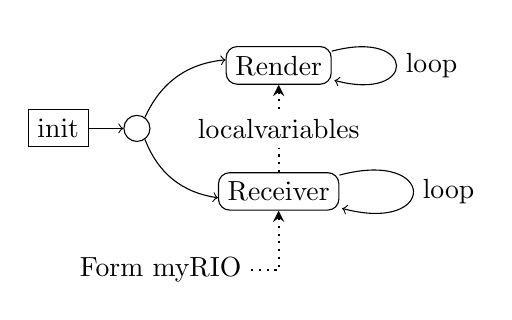
\begin{tikzpicture}
\tikzstyle{rounded} = [rectangle, rounded corners , minimum width=3mm, minimum height=1mm,text centered, draw=black]
\tikzstyle{round}=[circle, minimum width=0mm,draw=black]
\tikzstyle{square} = [rectangle, minimum width=1mm, draw=black]
\tikzstyle{empty}=[]

\usetikzlibrary{shapes.geometric, arrows}
\tikzstyle{arrow} = [thick,->,>=stealth]
\tikzstyle{dottarrow} = [thick, dotted,->,>=stealth]
\tikzstyle{dottline} = [thick, dotted,-,>=stealth]
\tikzstyle{noarrow}=[thick,-=,=stealth]

%nodes
\node (init) [square] {init};
\node (loop) [round, right of=init]{};
\node (render)[rounded, right of=loop, xshift=8mm, yshift=8mm ] {Render};
\node (rezive) [rounded, right of=loop, xshift=8mm, yshift=-8mm] {Receiver};
\node (datain) [empty, below of=rezive, xshift=-15mm]{Form myRIO};
\node (shared) [empty, below of=render, yshift=2mm]{localvariables};


%lines
%(Startnode)  edge [bend arrow]       node[text pos]  {text}          (target);
\path[->] 
(init) 		edge 								node[left]		{}			(loop)
(loop)		edge[bend left] 					node[left]		{}			(render)
(loop)		edge[bend right]					node[left]		{}			(rezive)
(render) 	edge[loop right]					node[right]		{loop}			(render)
(rezive) 	edge[loop right]					node[right]		{loop}			(rezive)
;
\draw [dottarrow] (datain) -| (rezive);
%\draw [dottarrow] (rezive) -- (render);
\draw [dottline] (rezive) -- (shared);
\draw [dottarrow] (shared) -- (render);

\end{tikzpicture}
        \includegraphics[scale=0.2]{./mesurment/data/Lidar_1ms_9_oclock_detection}
        \includegraphics[scale=0.2]{./mesurment/data/Lidar_10ms_9_oclock_detection}\\
        \includegraphics[scale=0.2]{./mesurment/data/Lidar_30ms_9_oclock_detection}
        \includegraphics[scale=0.2]{./mesurment/data/Lidar_40ms_9_oclock_detection}
    
 %\caption{blub}
  \caption{In this figure the only object that should be there is the object at $(x=-1, y=0)$ the rest is ghost except perhaps the one in the bottom because its the motor shaft that is going throw the cog and interferes with the sensor.}
  \label{fig:lidar-images}
\end{figure}


%\printbibliography
\end{document}